\chapter{Funzioni Crittografiche di Hash}
\section{Introduzione}
Una funzione di hash (o semplicemente hash o message digest) è una funzione unidirezionale (o one-way).
\begin{itemize}
\item è una funzione perché prende in input un messaggio e produce un output che dipende dal messaggio :
	\begin{itemize}
	\item h: $\{0, 1\}^{*} \rightarrow \{0, 1\}^{b}$
	\item $\{0, 1\}^{*}$: spazio delle stringhe binarie di lunghezza qualsiasi
	\item $\{0, 1\}^{b}$: spazio delle stringhe binarie di lunghezza b bit
	\item è considerata unidirezionale (one-way) perché è impraticabile capire quale input corrisponda ad un dato output
	\end{itemize}

Sia h() una funzione di hash, allora h() è una funzione di hash sicura se :
	\begin{itemize}
	\item resistenza alla preimmagine: fissato un hash $\hbar$ è
	computazionalmente impraticabile trovare un messaggio
	m tale che $h(m) = \hbar$
	\item resistenza alle collisioni: è computazionalmente
	impraticabile trovare due messaggi m1 e m2 aventi lo
	stesso digest h(m1) = h(m2), le proprietà precedenti implicano la seguente
	\item resistenza alla seconda preimmagine: dato un messaggio
	m, è computazionalmente impraticabile trovare un
	messaggio m’ avente lo stesso digest $h(m) = h(m’)$
	\end{itemize}
\end{itemize}

Si useranno i termini hash e message digest in modo intercambiabile; la funzione di hash del NIST è chiamata SHA-1: Secure Hash Algorithm mentre l’acronimo MD degli algoritmi MD2, MD4 e MD5 sta per Message Digest. Tutti gli algoritmi di digest/hash basicalmente fanno la stessa cosa: prendono in input un messaggio di lunghezza variabile, e restituiscono in output una quantità avente lunghezza prefissata.
Dato un messaggio m, il digest h(m) viene calcolato in modo deterministico. Tuttavia, l’output della funzione di hash dovrebbe apparire il più possibile casuale. Dovrebbe essere impossibile, senza applicare la funzione di
hash, predire ogni porzione dell’output e per ogni sottoinsieme (di posizioni) di bit nel digest h(m)
soltanto procedendo in modo esaustivo dovrebbe essere possibile ottenere due messaggi m1 e m2 tali che h(m1) e
h(m2) presentino gli stessi bit in quelle posizioni.
Perciò una funzione di hash sicura con n bit dovrebbe essere derivabile da una funzione di hash con più di n
bit prendendo un arbitrario sottoinsieme di n bit dal digest più grande.
Chiaramente, ci sono molti messaggi distinti che sono mappati in uno stesso digest h(m); m ha lunghezza arbitraria, mentre il digest h(m) ha una lunghezza prefissata, ad esempio 128 bit.
Se m ha una lunghezza di 1000 bit e h(m) di 128 bit ci sono in media 2872 messaggi che sono mappati in uno
stesso digest  dopo molti tentativi, due messaggi aventi lo stesso digest si trovano sicuramente.
Tuttavia, per “molti tentativi” si intende un numero talmente grande che è di fatto impossibile
considerando una buona funzione di digest a 128 bit, è necessario provare approssimativamente
$2^{128}$ possibili messaggi prima di ottenere un messaggio avente un particolare digest, o
$2^{64}$ messaggi prima di trovarne due aventi lo stesso digest ; trovare cioè due messaggi che collidono.

\section{Esempio di Applicazioni}
Un’applicazione delle funzioni di hash crittografiche è il calcolo dell’impronta digitale di
un programma o di un documento di cui si desiderano monitorare eventuali modifiche :
se il message digest h(p) del programma p è noto e se h(p) è memorizzato in modo sicuro (cioè non può essere
modificato da utenti non autorizzati) allora nessun utente non autorizzato può modificare p
senza essere scoperto perché non sarà in grado di trovare un diverso programma p’ tale che h(p’) = h(p).
Quindi sia h:$\{0, 1\}^{*} → \{0, 1\}^{b}$ una funzione di hash siano $m_{1}, m_{2}, …, m_{N}$ N messaggi arbitrariamente
scelti in ${0, 1}^{*}$. \\
\textbf{DOMANDA}: quanto deve valere N per avere una probabilità del $50\textdiscount$ che due messaggi $m_{i}, m_{j}$ abbiano lo stesso hash?

Una prima stima di N (affinché ci sia il 50\textdiscount di possibilità di collisione), per difetto, è la seguente :
\begin{itemize}
\item $k = 2^{b}$: numero totale di possibili hash
\item $\frac{1}{k}$ : probabilità che una coppia di messaggi collida
\item $\textbf{Ipotesi}$: gli eventi considerati sono mutuamente esclusivi 
	\begin{itemize}
		\item $\Pr\{h(mi) = h(mj) \textit{OR} h(mp) = h(mq)\} = \Pr\{h(mi) = h(mj)\} + \Pr\{ h(mp) = h(mq)\}$
	\end{itemize}
\end{itemize}
 
A rigore tale ipotesi non è soddisfatta, molti eventi hanno intersezione non nulla, perciò la stima ottenuta della probabilità è per eccesso e ciò si traduce in una stima per difetto di N $(\Pr\{E1 OR E2\} = \Pr\{E1\} + \Pr\{E2\} – \Pr\{E1 \bigcap E2\})$.
Si ha una probabilità del $50\textdiscount$ se si considerano $k/2$ coppie, perciò $N(N – 1)/2 = k/2$ e ipotizzando $N >> 1$ si ha $N = k^{1/2} = 2^{b/2}$.

Una seconda stima, più accurata di N è la seguente:
\begin{itemize}
\item P: probabilità che almeno una coppia di messaggi collida
\item $P^{*}$: probabilità che tutte le coppie di messaggi abbiano digest diversi, quindi $P = 1 - P^{*}$
\item \textbf{Ipotesi}: gli eventi considerati sono indipendenti
	\begin{itemize}
		\item $\Pr\{h(mi) \neq h(mj) \textit{AND} h(mp) \neq h(mq)\} = \Pr\{h(mi) \neq h(mj)\} * \Pr\{ h(mp) \neq h(mq)\}$
	\end{itemize}
\end{itemize}

A rigore tale ipotesi non è soddisfatta, gli eventi non sono del tutto indipendenti quindi la stima ottenuta della probabilità P è per difetto e ciò si traduce in una stima per eccesso di N ($\Pr\{E1 AND E2\} = \Pr\{E1\} * \Pr\{E1|E2\}$).
Nella ipotesi di eventi indipendenti si ha $P = 1 – P^{*} = 1 – (1 – 1/k)^{\frac{N(N – 1)}{2}}$, e ipotizzando che k >> 1 si ottiene che $P \approx 1 – e^{– N(N – 1)/2k}$, ponendo pertanto $P\geq1/2 si ottiene che e^{– N(N – 1)/2k} \leqslant 1/2 = e^{–ln2}$; da cui si ottiene che $N(N – 1)/2 \geq (ln2)k$ e, ipotizzando che N >> 1, $N \geqslant (2ln2)^{1/2} \cdot k^{1/2} = (2ln2)^{1/2} \cdot 2^{b/2}$.

Una terza stima ancor più corretta si può ottenere utilizzando la modalità di calcolo utilizzata anche nel paradosso del compleanno :
\begin{itemize}
\item P: probabilità che almeno una coppia di messaggi collida
\item $P^{*}$: probabilità che tutte le coppie di messaggi abbiano digest diversi, quindi $P = 1 - P^{*}$
\item $k = 2^{b}$: numero di possibili hash
\end{itemize}
Si consideri inoltre la seguente notazione:
\begin{itemize}
\item $P_{2^{*}}$: la probabilità che h(m2) sia diverso da h(m1)
\item $P_{3^{*}}$: la probabilità che h(m3) sia diverso da h(m2) e h(m1)
\item ...
\item $P_{i^{*}}$: la probabilità che h(mi) sia diverso da h(mj), $\forall 1\leq j \leq i-1$
\item ...
\item $P_{N^{*}}$: la probabilità che h(mN) sia diverso da h(mj), $\forall 1\leq j \leq N-1$
\end{itemize}
Da tutto ciò segue che $P^{*}=P_{2^{*}}*P_{3^{*}}*...*P_{i^{*}}*...*P_{N^{*}}=
(k – 1)/k*(k – 2)/k*...*(k – N + 1)/k = \frac{k!}{(k^{N}*(k – N)!)}\Rightarrow P^{*} = \frac{k!}{(k^{N}*(k – N)!)}$.
Questa è la stima esatta di $P^{*}$, si nota che il precedente valore di $P^{*}$ si può approssimare con $1 – e^{– N(N – 1)/2k}$.

\section{Lunghezza di un messaggio di Digest}
Quanti bit deve avere l’output di una funzione di hash in modo tale che nessuno sia in grado di trovare due messaggi aventi lo stesso digest?
Se il digest ha b bit, per trovare due messaggi aventi lo stesso digest, è necessario considerare circa $2^{b/2}$ messaggi, se il digest è lungo 64 bit, la ricerca esaustiva in uno spazio di circa $2^{32}$ elementi può essere fattibile mentre se il digest è lungo 128 bit si ritiene che una ricerca in uno spazio di $2^{64}$ elementi sia impraticabile dato l’attuale stato dell’arte.
Per quale ragione è importante che una funzione crittografica di hash sia resistente alle collisioni?
Il fatto che debba essere resistente alla preeimmagine è scontato, ma la resistenza alle collisioni è veramente necessaria?? Si, dato che in alcune circostanze riuscire a trovare due messaggi
con lo stesso digest può comportare dei seri problemi di sicurezza!!
Ad esempio, Alice genera una informazione $x_{A}$ e incarica Bob di calcolare un messaggio $m_{A}$ il cui contenuto deve dipendere da $x_{A}$ secondo criteri prestabiliti.
Una volta che Bob ha calcolato $m_{A}$ lo sottopone ad Alice che ne verifica l'integrità e calcola l'impronta $h(m_{A})$, la firma con la sua chiave privata e invia a Trudy il messaggio in chiaro $m_{A}$ e la sua firma.
Trudy legge il messaggio $m_{A}$ e la firma, controlla che la firma sia quella di Alice e verifica che tutto $m_{A}$ coincida con $h(m_{A})$.
\begin{figure}
	\begin{center}
	{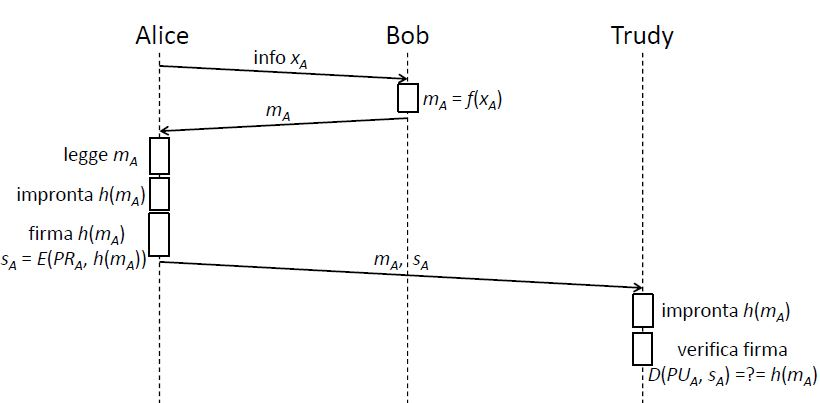
\includegraphics[height=13cm, width=13cm, keepaspectratio]{Immagini/Capitolo4/schema_hash_collisioni.JPG}}
	\end{center}
\end{figure}
Se la funzione non è resistente alla collisioni, Bob potrebbe trovare $m_{A1}$ tale che risulti $h(m_{A})= h(m_{A1})$.
Una volta che Alice ha firmato il messaggio, sostituisce $m_{A}$ con $m_{A1}$ e Trudy non si potrà mai accorgere di nulla.
\begin{figure}
	\begin{center}
	{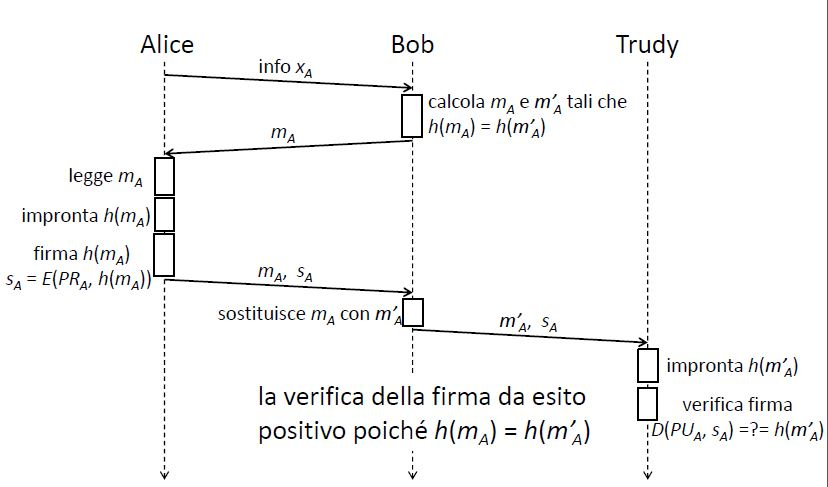
\includegraphics[height=13cm, width=13cm, keepaspectratio]{Immagini/Capitolo4/schema_hash_collisioni_1.JPG}}
	\end{center}
\end{figure}
Ma, per calcolare due messaggi con lo stesso hash, Bob può seguire il seguente approccio a forza bruta:
\begin{itemize}
\item dato xA, calcola prima il messaggio mA come desiderato da Alice;
\item genera un messaggio falsato $mA^{'}$;
\item esegue il test $h(mA)==h(mA^{'})$;
\item in caso negativo ritorna al punto 2;
\end{itemize}
con questo approccio a forza bruta, però, sono necessari circa $2^{b}$ tentativi, e non $2^{b/2}$!

\section{Impieghi degli Algoritmi di Hash}
Disponendo di un segreto condiviso, l'algoritmo di hash può "sostituire" un algoritmo di crittografia a chiave segreta in ogni suo impiego. (Autenticazione a chiave segreta, Calcolo di MAC, Cifratura e Decifratura).
\subsection{Message Digest per MAC}
Un possibile schema di autenticazione a chiave segreta (composta da "sfide") è il seguente
\begin{figure}
	\begin{center}
	{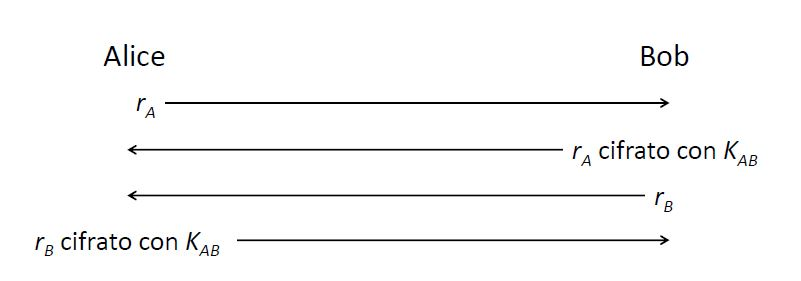
\includegraphics[height=13cm, width=13cm, keepaspectratio]{Immagini/Capitolo4/schema_autenticazione.JPG}}
	\end{center}
\end{figure}
Questo schema, purtroppo, presenta delle vulnerabilità...così come il seguente:
\begin{figure}
	\begin{center}
	{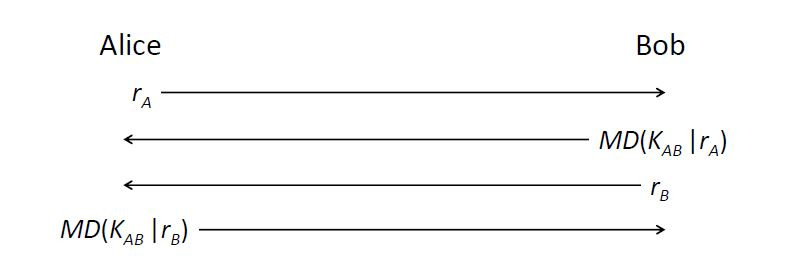
\includegraphics[height=13cm, width=13cm, keepaspectratio]{Immagini/Capitolo4/schema_autenticazione_md.JPG}}
	\end{center}
\end{figure}
Le vulnerabilità degli algoritmi di digest MD, sono note e facilmente attuabili in un possibile attacco.
Infatti, MD(m) è calcolabile da tutti coloro che conoscono m e l’algoritmo di digest MD senza conoscere la chiave 
segreta!!
Poiché, dall’input m si ottiene un messaggio mp avente lunghezza pari ad un multiplo intero di 512 bit ()mediante un opportuno padding che include, tra l’altro, la lunghezza originaria di m), mp viene decomposto in chunk (pezzi) da 512 bit il digest viene ottenuto mediante una procedura iterativa, quindi il digest all’n-esima iterazione dipende esclusivamente dall’n-esimo chunk e dal digest ottenuto all’(n – 1)-esima iterazione...il digest risultante di m è il digest ottenuto all’ultima iterazione.
Se un attaccante intercetta $\langle m, MD(K_{AB}|m) \rangle$ tra Alice e Bob, l'attaccante senza conoscere la chiave segreta $K_{AB}$ può calcolare il MAC di $\langle m^{+}, MD(K_{AB}|m^{*}) \rangle$ (dato che l'algoritmo di hash è noto) tramite l'ultimo messaggio intercettato. \\
Una possibile soluzione è che il segreto $K_{AB}$ sia messo in coda, a patto che l'algoritmo di hash sia molto resistente alle collisioni!! Un altra possibilità è quella di utilizzare come MAC un sottoinsieme arbitrario del digest MD, in questo caso, se il mio MAC è di soli 64 bit (invece di 128), l'attaccante potrebbe sempre ricostruire un messaggio da accodare...ma ha una possibilità su $2^{64}$ che il MAC ottenuto sia quello corretto.
\\
Una terza soluzione è quella di inserire il segreto $K_{AB}$ sia all'inizio che in coda del messaggio da mandare al digest MD, così che $K_{AB}$ in testa fornisca resistenza alle collisioni e $K_{AB}$ rende innocua la vulnerabilità insita negli algoritmi di hash.
Dato che ognuna delle soluzioni è equivalentemente corretta per ovviare al problema della vulnerabilità della funzione MD, per dare una piattaforma condivisa...una soluzione condivisibile da tutti, è stato introdotto il framework \textbf{HMAC} (keyed-Hash Message Authentication Code); l'algoritmo HMAC calcola due volte il digest del messaggio, e ogni volta inserisce in testa il segreto $K_{AB}$.
\subsection{Cifratura/Decifratura} 
Come faccio a cifrare con un algoritmo di hash? Devo utilizzare la funzione di hash potendo rendere tutto il processo invertibile, quindi introducendo lo XOR tra un chunk del messaggio e l' hash della chiave (genero un keypad) e ottengo un cifrario a flusso!!
\begin{figure}
	\begin{center}
	{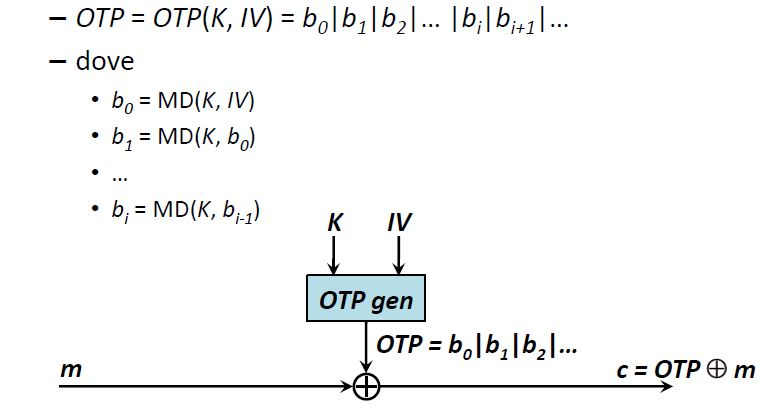
\includegraphics[height=13cm, width=13cm, keepaspectratio]{Immagini/Capitolo4/schema_cifratura_flusso.JPG}}
	\end{center}
\end{figure}

\subsection{Algoritmi di cifratura come algoritmi di hash}
Se un algoritmo di hash/digest, può essere utilizzato come un algoritmo di cifratura...può accadere il contrario?
In genere, questo principio è utilizzato (ad esempio) per la memorizzazione degli hash delle password in UNIX.
Ma come si modifica un algoritmo di cifratura che sia resistente alle collisioni?\\
Lo schema di funzionamento (minimale) è questa
\begin{figure}
	\begin{center}
	{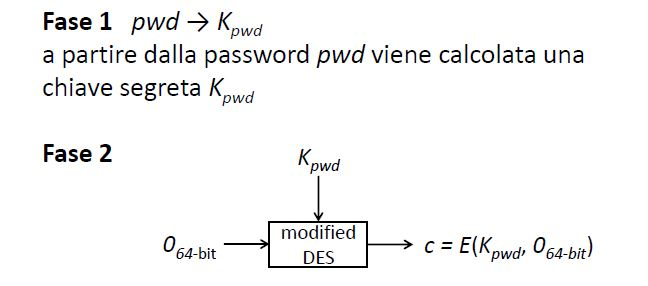
\includegraphics[height=13cm, width=13cm, keepaspectratio]{Immagini/Capitolo4/schema_des_come_hash.JPG}}
	\end{center}
\end{figure}
Ma questo schema funziona per soli messaggi corti e non è troppo resistente alle collisioni, sebbene $K_{PWD}$ sia ottenuta dalla pwd considerandone i primi 8 caratteri ed espansa con con i bit di parità per ogni gruppo di 8 bit.
Dato s il \textit{salt}, invero il numero di 12 bit ottenuto in modo pseudo randomico dalla pwd di ogni utente, la funzione h(pwd) si ottiene dal DES modificato che dipende dal valore di s (che determina quali bit  devono essere replicati nella fase di espansione di R da 32 a 48 bit). Infine il DES modificato è utilizzato con $K_{PWD}$ pr cifrare una costante 0 a 64 bit. Il risultato della cifratura e il salt, sono memorizzati per poter recuperare pwd.

\subsection{Hash di grandi messaggi con algoritmi di cifratura come hash}
Per l'algoritmo precedente, era stato sottolineato che era valido esclusivamente per messaggi corti.
Come si deve operare per estendere questi algoritmi a messaggi di lunghezza arbitraria?
Si può pensare di suddividere il messaggio $m = m_{1},m_{2},m_{3},...,m_{n}$, ogni $m_{i}$ viene utilizzato come input a un blocco in cascata di cifratura, alla fine della cascata ho realizzato un algoritmo di hash tramite cifratura...per un messaggio di lunghezza qualsiasi.\\
\begin{figure}
	\begin{center}
	{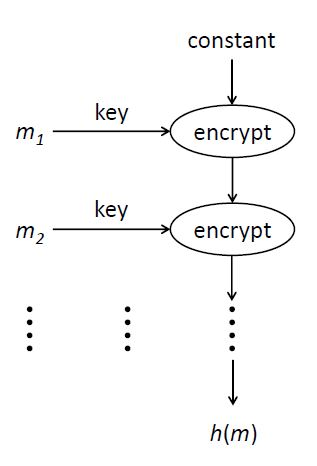
\includegraphics[height=10cm, width=10cm, keepaspectratio]{Immagini/Capitolo4/schema_des_come_hash_1.JPG}}
	\end{center}
\end{figure}
Purtroppo questo sistema soffre degli stessi problemi di cui soffriva il DES doppio, per ovviare ciò, basta rendere l'output di ogni blocco differente diverso dall'input del successivo, una possibile implementazione è la seguente
\begin{figure}
	\begin{center}
	{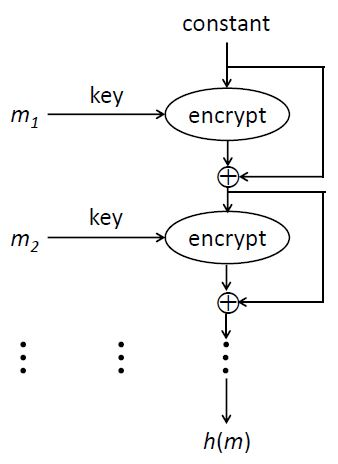
\includegraphics[height=10cm, width=10cm, keepaspectratio]{Immagini/Capitolo4/schema_des_come_hash_2.JPG}}
	\end{center}
\end{figure}

\subsection{Rainbow Tables (Opzionale)}
Le Rainbow tables sono un meccanismo per l'attacco di reverse hash. Le tables bilanciano memoria e sforzo computazionale, se fosse utilizzata solo memoria si avrebbero dei database troppo grandi per poter mappare tutte le immagini degli hash e se fosse utilizzata solo potenza computazionale servirebbe troppo tempo per poter trovare l'inverso di un hash.\\
Le Rainbow tables utilizzano delle funzioni di riduzione r(), la funzione di riduzione è una applicazione dallo spazio degli Hash allo spazio dei Plaintext, r() non è l'inversa di un algoritmo di hash; per questo, prima di avvicinarmi a una buona inversione dovrò concatenare fino a centinaia di iterazioni di $h(m) = k \longrightarrow r(k) = m^{'}$.
\begin{figure}
	\begin{center}
	{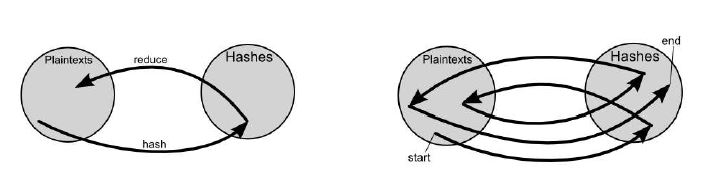
\includegraphics[height=10cm, width=10cm, keepaspectratio]{Immagini/Capitolo4/riduzione.JPG}}
	\end{center}
\end{figure}
Per popolare la table, si memorizzano solo il messaggio iniziale e il messaggio finale della catena. In questo modo, con una catena di 100 iterazioni (dato che le funzioni sono deterministiche) si risparmia uno spazio in memoria di 100 volte la grandezza della table, in confronto a memorizzare solo coppie $\langle plaintext, hash \rangle$.
Per recuperare un plaintext di un hash, si controlla se questo sia un endpoint di una qualsiasi delle catene (fase di lookup), se non lo fosse si controllano gli endpoint intermedi di ogni catena.
Appena recuperato l'hash giusto, si utilizza la catena determinata dall'inizio finchè non si trova l'hash di inizio; il messaggio che ha generato quell'hash sarà ciò che si cercava.
\begin{figure}
	\begin{center}
	{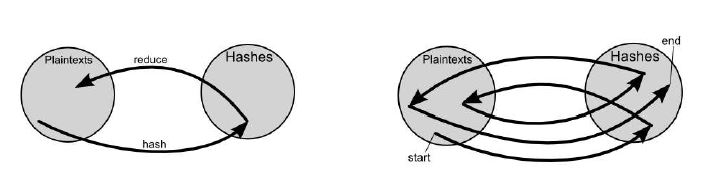
\includegraphics[height=10cm, width=10cm, keepaspectratio]{Immagini/Capitolo4/riduzione.JPG}}
	\end{center}
\end{figure}